% !TeX root = ../libro.tex
% !TeX encoding = utf8

\chapter{Introducción}  \label{ch:Introduccion_informatica}

\noindent Hoy en día vivimos en una sociedad en la que la tecnología se encuentra presente en prácticamente todas las tareas y disciplinas. Particularmente, en los últimos años hemos podido ver cómo el desarrollo \textbf{Inteligencia Artificial} ha permitido que tareas que antes se consideraban lentas o complicadas puedan realizarse rápidamente y con precisión con ayuda de un ordenador. En cambio, hay otras tareas que todavía resultan complicadas de resolver de forma rápida tanto para expertos en la materia como para ordenadores. Es dentro de este conjunto dónde se va a desarrollar el presente trabajo, pues como veremos a continuación y en posteriores secciones apenas hay publicaciones relacionadas con el tema. En particular se desarrollará en el ámbito de las ciencias forenses, que explicaremos a continuación.

\medskip

\noindent Las \textbf{ciencias forenses} son aquellas que aplican el método científico a hechos presuntamente delictivos con la finalidad de aportar pruebas a efectos judiciales. Dentro de este campo destacan principalmente dos disciplinas: 

\begin{itemize}
    \item La \textbf{Criminalística}: disciplina encargada del descubrimiento y verificación científica de presuntos hechos delictivos y quienes los cometen.
    \item La \textbf{Medicina Forense}: disciplina encargada de determinar el origen de las lesiones, las caisas de muerte o la identificación de seres humanos vivos o muertos.
\end{itemize}

\medskip

\noindent Dentro de la medicina forense se encuentra la \textbf{antropología forense}, que principalmente se encarga de la identificación de personas a partir de restos óseos. Y es en este ambiente dónde se encuentra el proceso que da sentido a este trabajo.


\section{Descripción del problema}

\noindent Los antropólogos forenses emplean diversas técnicas para la identificación de personas a partir de restos óseos como son la reconstrucción de huesos, el cotejo fotográfico con el cráneo o el análisis de imágenes. De entre estas técnicas, destaca la \textbf{Superposición Craneofacial} por ser la que se encuentra más relacionada con el fin de este trabajo. Se trata de una técnica de identificación forense mediante la cual se comparan imágenes de la persona difunta (imágenes se le denominan imágenes ante-mortem) con una representación 3D de un cráneo candidato, con el fin de determinar si el cráneo pertenece a la persona de las imágenes o no. En esta técnica se superpone el modelo 3D y la imagen del sujeto y se estima si son o no la misma persona. Para determinar esto se realiza un marcando puntos de referencia \textbf{de acuerdo a correspondencias morfológicas} tanto en la cara del sujeto en las imágenes como en el cráneo candidato, de manera que cada punto marcado sobre el rosto tiene un homólogo marcado sobre el cráneo. Estos puntos de referencia reciben el nombre de \textit{landmarks} y se denominan puntos craneométricos cuando se marcan sobre el cráneo y puntos cefalométricos cuando se marcan sobre el rostro. En caso de que el cráneo y la imagen pertenezcan a la misma persona existirá una correlación entre los dos tipos de \textit{landmarks} anteriores, o dicho de otra forma, en caso de que pertenezcan a la misma persona se podrá superponer el modelo del cráneo con los puntos marcados sobre la imagen marcada haciendo coincidir estos puntos.

\begin{figure}[!h]
    \centering
    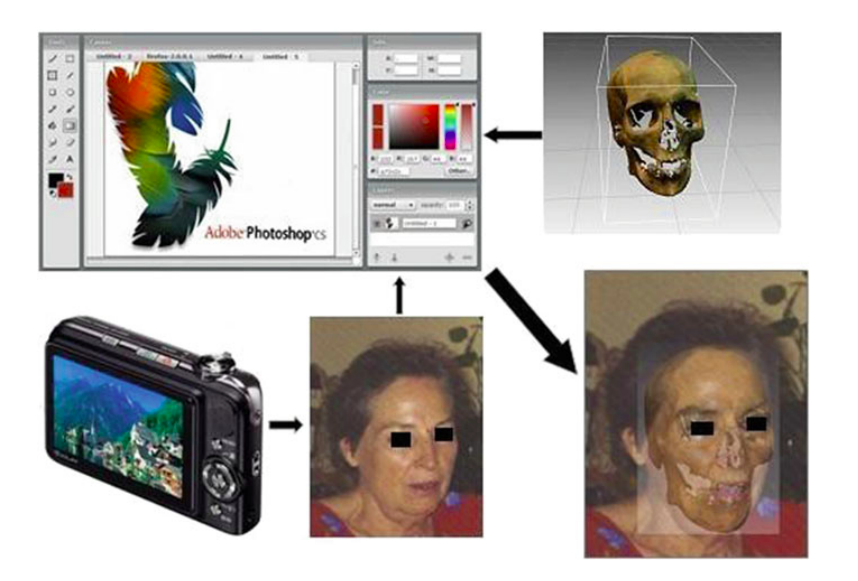
\includegraphics[width=0.8\textwidth]{img/ejemplo_SCF_intro.png}
    \caption{Ejemplo del proceso a seguir por el antropólogo forense en la superposición cráneo facial. Se parte de una imagen o varias de un sujeto, de un cráneo al que se le hace un modelado 3D y finalmente con ayuda de una herramienta como puede ser Photoshop se realizan las transformaciones necesarias sobre el modelo 3D hasta que coincida con la imagen. Imagen extraida de \cite{damas2020handbook}.}
\end{figure}

\medskip

\noindent Sin embargo, esta tarea no es sencilla por factores diversos a tener en cuenta como son la grasa, la calidad de la imagen y el tejido blando facial que separa el punto craneométrico de su homólogo cefalométrico y que se traduce en una ligera traslación del punto. El desplazamiento ocasionado por el tejido blando facial no es constante ni se produce siempre en la misma dirección, lo cual complica esta tarea. 

\begin{figure}[!h]
    \centering
    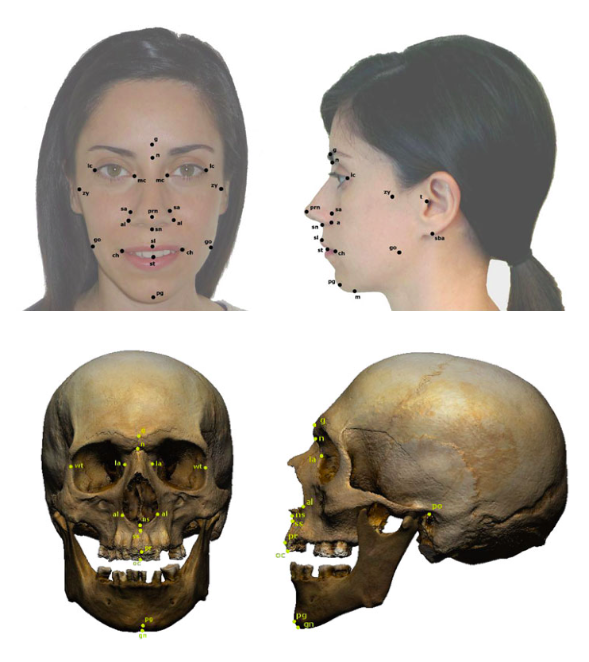
\includegraphics[width=0.97\textwidth]{img/marcado_landmarks.png}
    \caption{En este ejemplo podemos ver landmarks cefalométricos (imagen de la izquierda) y algunos de sus homólogos en los landmarks craneométricos de la imagen de la derecha. También podemos ver el efecto del tejido blando facial en la imagen de la izquierda en el desplazamiento de los puntos. Imagen extraida de \cite{damas2020handbook}.}
\end{figure}

\medskip Una vez determinados los landmarks, un algoritmo automático puede encargarse de realziar el solapamiento del cráneo 3D y la imagen 2D.

\section{Motivación}

Tradicionalmente, este proceso del marcado de landmarks es esencialmente manual y complicado de replicar, y pese a los avances actuales que se están llevando a cabo para automatizar esta tarea \cite{Huete2015PastPA}, la identificación de \textit{landmarks} sigue realizándose a mano normalmente. Sin embargo en la identificación de landmarks \textbf{craneométricos} podemos encontrar algunos trabajos publicados como \cite{bermejo2021automatic} que permiten una atomatización de esta parte del proceso. En este contexto, el presente trabajo se centrará en esta etapa del marcado de \textbf{landmarks cefalométricos} (en las imágenes ante-mortem), de manera que se intentará automatizar este proceso.

\medskip

\noindent El algoritmoque buscamos, debido a la importancia de la tarea que debe cumplir, tiene que cumplir con unos requisitos mínimos deseables: 

\begin{itemize}
    \item Debe ser un método \textbf{robusto}, en el sentido de que debe abarcar todos los posibles casos y variaciones del problema. En nuestro caso se traduce en saber lidiar con imágenes frontales, de perfil o $3/4$ junto con otros factores como la calidad de la imagen, iluminación y oclusiones parciales. En todos los casos anteriores, el algoritmo debería tener un buen comportamiento.
    
    \medskip

    \noindent Esta propiedad es deseable porque generalmente, en los problemas forenses reales, no se dispone de una amplia variedad de imágenes de la persona desaparecida, en algunos casos sólo se dispone de unas pocas imágenes y no todas van a ser frontales y con buena calidad e iluminación.

    \item Capaz de operar con un \textbf{pequeño conjunto de datos}, ya que como hemos comentado anteriormente, se dispone generalmente de pocas imágenes para realizar el marcado de landmarks.
    \item Debe proporcionar una solución \textbf{correcta} o al menos lo más correcta posible.  
    \item Debe ser \textbf{completo}, contando con todos los recursos necesarios para poder operar.
    \item Debe ser \textbf{eficaz} y \textbf{eficiente}. Buscamos acelerar el proceso del marcado de landmarks considerablemente a la par que conseguir resolver el objetivo principal.
\end{itemize}

\noindent Remarcamos que la intención no es reemplazar al experto en su labor del marcado de landmarks sino proporcionar una ayuda para acelerar el proceso, que hoy en día se sigue considerando un proceso lento.

\medskip 

\noindent Debido a que el algoritmo va a operar con imágenes, buscamos una solución dentro del área de la \textbf{visión por computador}. Actualmente existen  multitud de trabajos relacionados con el marcado de landmarks en imágenes dentro de este área, la mayoría usando algoritmos de \textbf{deep learning} y enfocadas al reconocimiento de individuos en imágenes. Los landmarks que marcan en estas propuestas no siguen correspondencias morfológicas, y dependen únicamente de la estructura facial del individuo. Dichos algoritmos son entrenados con grandes bases de datos de imágenes etiquetadas y actualmente se obtienen excelentes resultados en este tipo de problemas.


\section{Objetivos}

\noindent Con todo lo mencionado anteriormente nuestro objetivo principal será adaptar el framework \textbf{3FabRec} \cite{browatzki20203fabrec} para la detección de landmarks cefalométricos empleando una base de datos forense con pocas imágenes. Para lograr este objetivo se pretenden realizar también los siguientes objetivos menores: 


\endinput
%------------------------------------------------------------------------------------
% FIN DEL CAPÍTULO. 
%------------------------------------------------------------------------------------


